% Chapter 1equation results in
%
% \begin{equation}
% \Del \cross ( \Del \cross
\chapter{Physical Problem} % Write in your own chapter title
\label{PhysicalProblemChapter}
\lhead{Chapter 2. \emph{Physical Problem}} % Write in your own chapter title to set the page header

\section{Maxwell's equations}

%\begin{itemize}
%  \item show four equations - introduce them one at a time (Gauss, Ampere etc...)
%	\item specify equations (system of PDEs, linear conservation form)
%  \item consititive equations
%  \item discuss validity (linear, homogenous, isotropic)
%	\item Curl/Divergence only -> conservation form (this will be a discussion point, because the non-curl equations are not necessarily satisfied. My solution could violate the non-curl stuff....)
%	\item Differential vs integral formulation - why this form?
%  \item TE + TM decoupling (call it reductions to 2D or 1D)
%\end{itemize}
%

In this chapter, Maxwell's equations of classical electrodynamics in both integral and differential form will be introduced. In all the systems we consider the wavelength of radiation is sufficiently large, with respect to atomic scale variations in the medium, that a macroscopic approach is justified and quantum mechanical effects can be neglected. Constitutive equations will be introduced for linear, isotropic material both with and without dispersive effects. Following this, the Drude model will be used to incorporate the constitutive equations for dispersive media into Maxwell's equations in a formulation suitable for efficient numerical calculations. The conditions which must be satisfied at material interfaces will be derived and various forms of Maxwell's equations discussed.

The classical theory of electrodynamics decribes the time evolution of light using James Clerk Maxwell's unification of the equations of electrodynamics \cite{Maxwell:1863ur}, for a more detailed discussion of Maxwell's equations see \cite{Balanis:ui,Jackson:490457}. The resulting coupled equations which govern the time evolution of electromagnetic waves in a medium, are known collectively as Maxwell's equations and expressed in integral form in SI units as
\begin{subequations}
\begin{align}
    \int_{\partial S} \mathbf{E}(\mathbf{x},t) \cdot \mathrm{d}\boldsymbol{\ell}  &= - \frac{d}{dt} \int_{S} \mathbf{B}(\mathbf{x},t) \cdot \mathrm{d}\mathbf{S}, \label{eq:maxwell-faraday-integral} \\
    \int_{\partial S} \mathbf{B}(\mathbf{x},t) \cdot \mathrm{d}\boldsymbol{\ell} &= \mu_0 \varepsilon_0 \frac{d}{dt} \int_{S} \mathbf{E}(\mathbf{x},t) \cdot \mathrm{d}\mathbf{S} +  \mu_0 \int_{S} \mathbf{J}(\mathbf{x},t) \cdot \mathrm{d}\mathbf{S}, \label{eq:maxwell-ampere-integral} \\
    \int_{\partial V} \mathbf{D}(\mathbf{x},t)\cdot\mathrm{d}\mathbf{S} &= \int_V \rho \,\mathrm{d}V, \label{maxwell-gauss-integral} \\
    \int_{\partial V} \mathbf{B}(\mathbf{x},t)\cdot\mathrm{d}\mathbf{S} &= 0, \label{maxwell-gauss-magnetism-integral}
\end{align}
\end{subequations}
where $\mathbf{x}$ is the position vector, $t$ is time, $\epsilon_0$ is the permittivity of free space, $\mu_0$ is the permeability of free space and the 3-dimensional vector quantities $\mathbf{E}$, $\mathbf{H}$, $\mathbf{D}$ and $\mathbf{B}$ denote respectively the electric field, magnetic field, electric displacement and magnetic induction.
% QUOTE: both denote sources due to free charges in the system
$V$ denotes any closed volume while the infinitesimal integration elements $\mathrm{d}l$, $\mathrm{d}\mathbf{S}$ and $\mathrm{d}V$ are respectively a line element, vector surface element and volume element.
% "In regions where the material parameters are differentiable"... -> but hang on! The material parameters are not involved here. What restrictions are the for using Stokes' Theorem?
By applying Stokes' Theorem to equations \ref{eq:maxwell-faraday-integral} and \ref{eq:maxwell-ampere-integral} and Gauss's law to \ref{maxwell-gauss-integral} and \ref{maxwell-gauss-magnetism-integral}, the equations in differential form are readily obtained as
\begin{subequations}
\label{maxwells-equations-diff}
\begin{align}
    \nabla \times \mathbf{E}(\mathbf{x},t) + \frac{\partial }{\partial t} \mathbf{B}(\mathbf{x}, t) &= 0, \label{maxwell-faraday} \\
    \nabla \times \mathbf{H}(\mathbf{x},t) - \frac{\partial }{\partial t} \mathbf{D}(\mathbf{x}, t) &= \mathbf{J}(\mathbf{x},t), \label{maxwell-ampere} \\
    \nabla \cdot \mathbf{D} (\mathbf{x},t) &= \rho(\mathbf{x},t), \label{maxwell-gauss-1}, \\
    \nabla \cdot \mathbf{B} (\mathbf{x},t) &= 0, \label{maxwell-gauss-2} .
\end{align}
\end{subequations}
The four equations in \ref{maxwells-equations-diff} are known respectively as Ampere's law with Maxwell's correction, Faraday's law, Gauss' law and Gauss' law for magnetism. Equations \ref{maxwell-ampere} and \ref{maxwell-faraday}, known as Maxwell's curl equations, determine the evolution of the vector fields in time, and Maxwell's divergence conditions, \ref{maxwell-gauss-1} and \ref{maxwell-gauss-2}, are constraints on the vector fields which must be satisfied at all times.

\subsection{Conservation of charge}

Conservation of charge can be derived directly from Maxwell's equations. The vector identity
\begin{equation}
\label{eq:vector-identity-1}
\nabla \cdot ( \nabla \times \mathbf{A} ) = 0,
\end{equation}
which holds for any vector field $\mathbf{A}$, is substituted into the expression obtained by taking the divergence of both sides of Ampere's law, equation \ref{maxwell-ampere}, giving:
$$
- \frac{\partial}{\partial t} \nabla \cdot \mathbf{D}(\mathbf{x},t) = \nabla \cdot \mathbf{J}.(\mathbf{x},t) .
$$
By substituting Gauss' law, \ref{maxwell-gauss-1}, into this equation we obtain the following conservation equation for charge
\begin{equation}
\label{eq:maxwell-charge-conservation-2}
\nabla \cdot \mathbf{J}(\mathbf{x},t) + \frac{\partial \rho (\mathbf{x},t) }{\partial t} = 0 .
\end{equation}
Taking the divergence of Amperes equation \ref{maxwell-ampere}, and removing the curl term by recalling the identity \ref{eq:vector-identity-1}, results in

$$
\nabla \cdot \frac{\partial \mathbf{D}(\mathbf{x}, t)}{\partial t} = - \nabla \cdot \mathbf{J}(\mathbf{x},t),
$$

which can be rewritten using the conservation of charge equation, \ref{eq:maxwell-charge-conservation-2}, as

$$
\nabla \cdot \frac{\partial \mathbf{D}(\mathbf{x}, t)}{\partial t} = - \frac{\partial \rho (\mathbf{x},t)}{\partial t}.
$$

Following a similar procedure using equation \ref{maxwell-faraday} results in

$$
\nabla \cdot \frac{\partial \mathbf{B}(\mathbf{x}, t)}{\partial t} = 0
$$

Thus provided the initial conditions satisfy equation Maxwell's divergence conditions, \ref{maxwell-gauss-1} and \ref{maxwell-gauss-2}, and the conservation of charge equation, \ref{eq:maxwell-charge-conservation-2}, is satisfied at all times then if the system is evolved in time using Maxwell's curl equations alone the divergence conditions will be implicitly satisfied at all times.

\section{Constitutive equations}

Clearly, Maxwell's equations in differential form, \ref{maxwells-equations-diff}, cannot be solved alone. The system of equations is closed by macroscopic constitutive laws, which characterise the interaction between the medium and the electromagnetic fields. In general, for materials which do not exhibit ferromagnetic or ferroelectric behaviour the consitutive laws take the form
\begin{subequations}
    \label{constitutive-general}
    \begin{align}
        \mathbf{D}(\mathbf{x},t) &= \epsilon_0 \mathbf{E}(\mathbf{x},t) + \mathbf{P} \label{constitutive-general-E} \\
        \mathbf{B}(\mathbf{x},t) &= \mu_0 \mathbf{H}(\mathbf{x},t) + \mathbf{M}
    \end{align}
\end{subequations}
where $\epsilon_0$ and $\mu_0$ are the permittivity and permeability of free space, related by $c_0 = 1/ \sqrt{\epsilon_0 \mu_0}$, where $c_0$ is the speed of light in vacuum. The polarisation density, $\mathbf{P}$, and the magnetisation density, $\mathbf{M}$,
may each depend on any of the quantities $\mathbf{E}$, $\mathbf{H}$, $\mathbf{x}$ and $t$. However, for a given material the dependence may be complicated, and in particular may be one or more of the following: non-local in space, non-local in time, non-linear, or anisotropic. Despite this, the response of many materials can be accurately approximated as linear, isotropic and non-dispersive. In this case the relationship between $\mathbf{P}$ and $\mathbf{E}$ and that between $\mathbf{M}$ and $\mathbf{H}$ is linear, and the constitutive equations, \ref{constitutive-general}, can be rewritten in the simple form
%, are respectively the electric and magnetic dipole moment per unit volume in the medium. The polarisation and magnetisation densitites
%
\begin{subequations}
    \label{constitutive-linear}
    \begin{align}
        \mathbf{D}(\mathbf{x},t) = \epsilon_0 \epsilon_r(\mathbf{x}) \mathbf{E}(\mathbf{x},t), \label{constitutive-linear-D} \\
        \mathbf{B}(\mathbf{x},t) = \mu_0 \mu_r(\mathbf{x}) \mathbf{H}(\mathbf{x},t),
    \end{align}
\end{subequations}
%
where the material response is completely characterised by two dimensionless scalars: the relative permittivity, $\epsilon_r$, and the relative permeability, $\mu_r$.

Several metals of interest in photonics, such as gold, silver and aluminum, have relative permittivites which vary significantly as a function of frequency in the visible and infra-red regions of the electromagnetic spectrum \cite{Ordal:1983bg}.
% cite{Maier:5SXqSjV8} -> copied
This frequency dependence of permittivity is manifested in the time domain as a convolution integral in time, which appears in the constitutive equations \ref{constitutive-general} \cite{Jackson:490457}.
This phenomenum, known as dispersion, occurs in all materials due to the finite time required for charged particles in a material to reach new equilibrium position in the presence of an applied electric field.
These cases neccessitate a more sophisticated model of polarisation of a medium in response to an electric field. For metals where the effects of interband electron transitions are negligible, the Drude of model of solids, proposed in 1900 \cite{Drude:1900hg} based on the kinetic theory of gases, is sufficient to provide accurate results. In cases where interband transitions are significant a more sophisticated model such as the Drude-Lorentz model may be required \cite{Fox:2001wm,Taflove:1989ds}.

\subsubsection{Drude model}
\label{sub:The Drude Model}

% \begin{itemize}
% 	\item what is dispersion
% 	\item materials with free electrons exhibit strong dispersion
%   \item required for fast-varying fields in comparison to material response time (causal effects of polarisaiont)
% 	\item approaches - convolution intergral vs ADE
% 	\item Derivation [ Drude model in Freq domain -> Polarisaion -> FFT -> ADE -> coupled ODEs ]
%   \item Lorentz + more sophisticated models
% \end{itemize}
%% *** ## "Polarization density also describes how a material responds to an applied electric field as well as the way the material changes the electric field, and can be used to calculate the forces that result from those interactions."
In this model the medium is composed of a lattice of fixed-position, positively charged ions bound by a delocalised sea of valence band free electrons \cite{Ashcroft:2005wp,Bandyopadhyay:1503732}. The free electrons, following the kinetic theory of ideal gases, are non-interacting, independent particles, described by Newtonian mechanics. In the presence of the electric field, $\mathbf{E}$, the ions are fixed and only the valence electrons are displaced from their zero-field equilibrium positions.
%*** "The induced polarisation due to frequency-dependent electron movement leads to a frequency-dependent polarisation (dispersion)" - ref Maier
%
%Electron-ion collisions are random events, with a probability $dt / \tau$ (tau is the inv of gamma) - following which the electron velocities are independent of velocities prior to collision.

In the Drude model, $\mathbf{P}$ arises from two independent contributions, $\mathbf{P} = \mathbf{P}_{\infty} + \mathbf{P}_e$. The background polarisation, $\mathbf{P}_{\infty}$, is due to the fixed-position ions and is frequency independent. The subscript in this quantity indicates that $\mathbf{P} \to \mathbf{P}_{\infty}$ in the limit $\omega \to \infty$. The free electron polarisation, $\mathbf{P}_e$, is due to the delocalisation of free electrons in the presence of an electric field.

Since the ions are fixed in the Drude model, $\mathbf{P}_{\infty}$ is expected to be independent of frequency. This can be expressed in the frequency domain as a direct proportionality between $\mathbf{P}_{\infty}$ and $\mathbf{E}$, therefore equation \ref{constitutive-general-E} can be rewritten as
%
\begin{equation}
\label{eq:constitutive_equations_drude_model}
\hat{\mathbf{D}}(\mathbf{x},\omega) = \epsilon_0 \epsilon_{\infty}  \hat{\mathbf{E}}(\mathbf{x}, \omega) + \hat{\mathbf{P}}_e(\mathbf{x},\omega) ,
\end{equation}
%
where $\epsilon_{\infty}$ is the permittivity in the infinite frequency limit, and $\omega$ is the frequency variable. Here, and for the remainder of this section, a circumflex is used to denote the frequency domain representation of a time domain quantity.

Transforming equation \ref{eq:constitutive_equations_drude_model} directly to the time domain would lead to a convolution integral, which would be difficult to solve numerically. First multiplying equation \ref{eq:constitutive_equations_drude_model} by $ -i \omega$ gives
\begin{equation}
\label{eq:constitutive_equations_drude_model_derivative_FD}
- i \omega \hat{\mathbf{D}} = -i \omega \epsilon_0 \epsilon_{\infty} \hat{\mathbf{E}} + \hat{\mathbf{J}}_p,
\end{equation}
where we have substituted for $i \omega \hat{\mathbf{P}}_e$, using
\begin{equation}
\label{eq:drude-free-elect-current-defn}
\hat{\mathbf{J}}_p(\omega) = i \omega \hat{\mathbf{P}}_e(\omega) ,
\end{equation}
the definition of the current due to free electron polarisation.
Equation \ref{eq:constitutive_equations_drude_model_derivative_FD} can then now be transformed to the time domain to obtain the ordinary differential equation
\begin{equation}
\label{eq:constitutive_equations_drude_model_derivative_TD}
\frac{\partial}{\partial t} \mathbf{D} = \epsilon_0 \epsilon_{\infty} \frac{\partial}{\partial t} \mathbf{E} + \mathbf{J}^p .
\end{equation}
By substitution into equation \ref{eq:constitutive_equations_drude_model_derivative_TD} into Ampere's equation, \ref{maxwell-ampere}, we obtain the expressions
\begin{subequations}
\label{eq:drude-ampere}
    \begin{align}
        \nabla \times \mathbf{H}(\mathbf{x},t) - \frac{\partial }{\partial t} \mathbf{D}_{\infty}(\mathbf{x}, t) &= \mathbf{J}(\mathbf{x},t) + \mathbf{J}^p(\mathbf{x},t) , \\
        \mathbf{D}_{\infty}(\mathbf{x}, t) &= \epsilon_0 \epsilon_{\infty} \mathbf{E}(\mathbf{x}, t),
    \end{align}
\end{subequations}
where $\mathbf{D}_{\infty}$ has been introduced to maintain a consistent form with Maxwell's equations, as given in \ref{maxwells-equations-diff}.

To close the system of equations an expression for $\mathbf{J}^p$ is required. Since this is the current due to movement of free electrons, we begin by writing the Newtonian equation of motion of a free electron in the presence of an applied electric field, as
\begin{equation}
\frac{d^2}{dt^2}\mathbf{x}(t) + \gamma \frac{d}{dt} \mathbf{x}(t) = \frac{q}{m_e}\mathbf{E}(\mathbf{x}(t),t),
\label{equations-of-motion-electron}
\end{equation}
where $\gamma$ is a damping coefficient or collision frequency, $m_e$ is the mass of an electron, $q$ is the charge of an electron, $\mathbf{E}(\mathbf{x},t)$ is the applied electric field and $\mathbf{x}$ is the displacement of the electron from its zero-field equilibrium position. Given that the polarisation field due to electron movement is given by $ \mathbf{P}_e(t) = - n q \mathbf{x}(t)$, where $n$ is the electron density in the medium, then equation \ref{equations-of-motion-electron} can be rewritten as
\begin{equation}
\label{polarisation-from-P}
\frac{d^2}{dt^2}\mathbf{P}_e(t) + \gamma \frac{d}{dt} \mathbf{P}_e(t) = \epsilon_0 \omega_p^2 \mathbf{E}(\mathbf{x}(t),t),
\end{equation}
where $\omega_p = \sqrt{\frac{n q^2}{m_e \epsilon_0}}$ is known as the plasma frequency.
%We consider a single frequency in the frequency domain by selecting a monochromatic field of the form
%$$
%\mathbf{E}(\mathbf{x},t) = \hat{\mathbf{E_0}} e^{- i \omega t}
%$$
%with a known angular frequency $w$ and constant amplitude $\hat{\mathbf{E}}$.
%
Transforming equation \ref{polarisation-from-P} to the frequency domain we obtain the following:
\begin{equation}
\label{polarisation-from-P-FD}
( i \omega )^2 \hat{\mathbf{P}}_e(\omega) + \gamma (i \omega) \hat{\mathbf{P}}_e(\omega) = \epsilon_0 \omega_p^2 \hat{\mathbf{E}}(\mathbf{x},\omega),
\end{equation}
where $i$ is the imaginary unit and $\hat{\mathbf{E}}$ is a harmonic electric field given by $\mathbf{E}(\mathbf{x},t) = \hat{\mathbf{E}}(\mathbf{x}) e^{- i \omega t }$.

Substituting equation \ref{eq:drude-free-elect-current-defn} into \ref{polarisation-from-P-FD} gives
\begin{equation}
    \label{eq:pol-current-freq-domain}
  i \omega \hat{\mathbf{J}}_p(\omega) + \gamma \hat{\mathbf{J}}_p(\omega) = \epsilon_0 \omega_p^2 \hat{\mathbf{E}}(\omega) ,
\end{equation}
which, when transformed to the time domain, results in the following ordinary differential equation:
\begin{equation}
  \frac{d}{dt} \mathbf{J}^p(\mathbf{x})+ \gamma \mathbf{J}^p(\mathbf{x}) = \epsilon_0 \omega_p^2 \mathbf{E}(\mathbf{x},t).
  \label{pol-current-ADE}
\end{equation}

The complete set of coupled equations for a Drude model of dispersive material, including the modification shown in \ref{eq:drude-ampere} and \ref{pol-current-ADE}, is given by
\begin{subequations}
    \label{eq:dispersive-maxwell-system}
    \begin{align}
        \nabla \times \mathbf{E}(\mathbf{x},t) + \frac{\partial }{\partial t} \mathbf{B}(\mathbf{x}, t) &= 0, \\
        \nabla \times \mathbf{H}(\mathbf{x},t) - \frac{\partial }{\partial t} \mathbf{D}_{\infty}(\mathbf{x}, t) &= \mathbf{J}(\mathbf{x},t) + \mathbf{J}^p(\mathbf{x},t), \\
        \mathbf{D}_{\infty}(\mathbf{x},t) &= \epsilon_0 \epsilon_{\infty}(\mathbf{x}) \mathbf{E}(\mathbf{x},t), \\
        \mathbf{B}(\mathbf{x},t) &= \mu_0 \mu_r(\mathbf{x}) \mathbf{H}(\mathbf{x},t), \\
        \frac{d \mathbf{J}^p(\mathbf{x})}{dt} + \gamma \mathbf{J}^p(\mathbf{x}) &= \epsilon_0 \omega_p^2 \mathbf{E}(\mathbf{x}, t) . \label{eq:maxwell-dispersive-ADE}
    \end{align}
\end{subequations}
%
We note that the dispersive equations, \ref{eq:dispersive-maxwell-system}, reduce to the non-dispersive form of Maxwell's curl equations, \ref{maxwell-ampere} and \ref{maxwell-faraday}, and the constitutive equations for a non-dispersive dielectric given in \ref{constitutive-linear}, when $\mathbf{\epsilon}_r = \mathbf{\epsilon}_{\infty}$ and $\mathbf{J}^p = 0$. Dispersive behaviour is accounted for by the addition of an auxiliary differential equation (ADE) \cite{Taflove:1989ds,Niegemann:2009uv,Ji:2007dl}, given by \ref{eq:maxwell-dispersive-ADE}, coupled to Maxwell's equations by an additional polarisation current, $\mathbf{J}^p$.

Some insight into the behaviour of Drude metals can be obtained by looking at the relative permittivity obtained in the frequency domain. First, the constitutive equation \ref{polarisation-from-P-FD} can be rearranged to obtain the polarisation due to free electrons in the frequency domain,
\begin{equation}
\hat{\mathbf{P}}_e = - \frac{\epsilon_0 \omega_p^2}{\omega^2 - i \omega \gamma } \hat{\mathbf{E}}(\omega) .
  \label{eq:polarization-field-freq-domain}
\end{equation}
Using this expression, equation \ref{eq:constitutive_equations_drude_model} may be rewritten explicitly in the frequency domain as
\begin{equation}
    \begin{split}
    \hat{\mathbf{D}}(\mathbf{x},\omega) &= \epsilon_0 \left( \epsilon_{\infty} - \frac{\omega_p^2 }{\omega^2 - i \omega \gamma } \right) \hat{\mathbf{E}}(\omega) \\
                                        &= \epsilon_0 \hat{\epsilon}_r (\omega) \hat{\mathbf{E}}(\omega) ,
    \end{split}
\end{equation}
where $\hat{\epsilon}_r(\omega)$ is the effective permittivity of the metal. Figure \ref{fig:read-and-imag-effective-permittivity} shows the real and imaginary parts of $\hat{\epsilon}_r$, given by
\begin{subequations}
\begin{align}
    Re\{ \hat{\epsilon}_r \} &= \epsilon_{\infty} - \frac{\omega_p^2}{\omega^2 + \gamma^2}, \\
    Im\{ \hat{\epsilon}_r \} &= \frac{\gamma \omega_p}{\omega ( \omega^2 + \gamma^2) } ,
\end{align}
\end{subequations}
plotted against normalised angular frequency $\omega / \omega_p$. We observe that at higher frequencies, due to reduced electron motion, the non-dispersive dielectric behaviour is recovered as $Re\{\hat{\epsilon}_r\} \to \epsilon_{\infty}$ and $Im\{\hat{\epsilon}_r\} \to 0$. For frequencies below $\omega_p$ however, the real and imaginary parts of the permittivity diverge significantly from the dispersive values. The positive values of the imaginary part result in an attenuation of the electric field amplitude in this region.

\begin{figure}[htbp!]
\begin{center}
    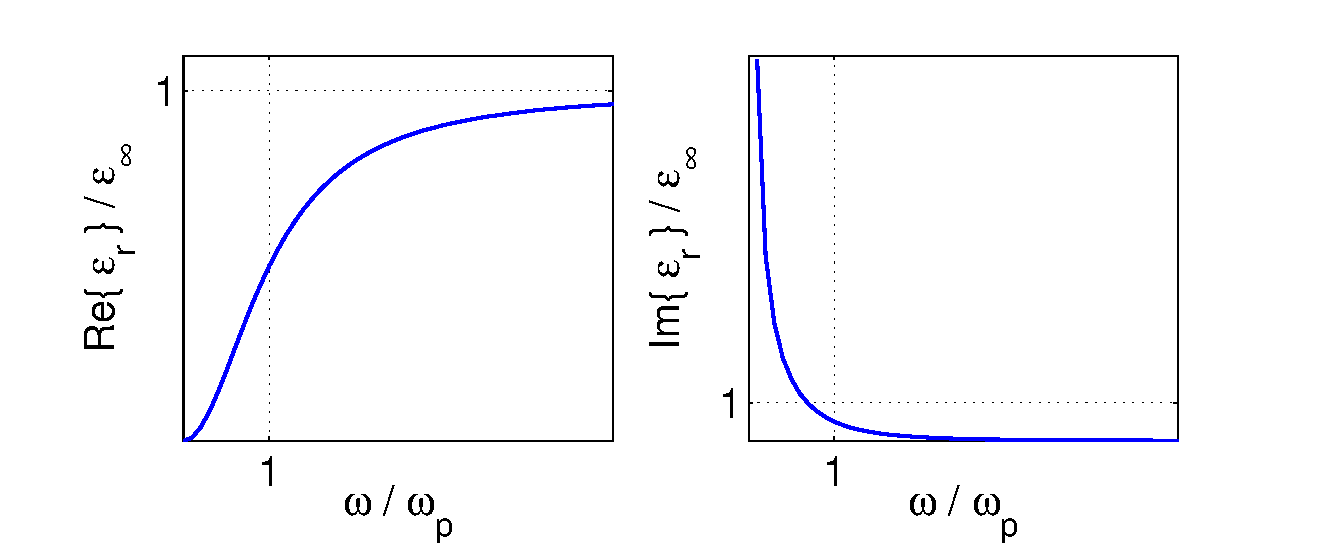
\includegraphics[scale=0.7]{Figures/Chapters/PhysicalProblem/drudePermittivity}
\end{center}
\caption{The real (left) and imaginary (right) parts of the dispersive frequency domain relative permittivity, $\hat{\epsilon}_r$, as obtained from Drude model.}
\label{fig:read-and-imag-effective-permittivity}
\end{figure}


%%%%%%%%%%%%%%%%%%%%%%%%%%%%%%%%%%%%%%%%%%%%%%%%%%%%%%%%%%%%%%%%%%%%%%%%%%%%%%%%%%%%%%%%%%%%%%%%%%%%%%%%%%%%%%%%%%%%%%%%%%%%%%%%%%%%%%%%%%%%%%%%%%%%%
%      More Dude Model Stuff
%%%%%%%%%%%%%%%%%%%%%%%%%%%%%%%%%%%%%%%%%%%%%%%%%%%%%%%%%%%%%%%%%%%%%%%%%%%%%%%%%%%%%%%%%%%%%%%%%%%%%%%%%%%%%%%%%%%%%%%%%%%%%%%%%%%%%%%%%%%%%%%%%%%%%
%
%TODO  - direct quote - IntriaPaper DGTD dispersive
%
%  When subjected to a constant external electric field $\mathbf{E}$ the displacement of the heavy valence ions from their equilibtrium position is assume to be negligable whilst the electrons move significantly from their equilibrium position in response to an externally applied field. This results in an additional electric field $\mathbf{P}$ due to material response to the applied field $\mathbf{E}$ orientated in the opposite direction resulting in a total field given by the electric displacement field $\mathbf{D}$ where:
% 
%  $$
%  \mathbf{D} = \epsilon_0 \mathbf{E} + \mathbf{P}
%  $$
% 
%  Note that usually the signs of $\mathbf{P}$ and $\mathbf{E}$ will be opposite - resulting in an induced field that opposes the applied field and consequentially a reduced field in the medium.
% 
%  % TODO: Is it accurate to describe the displacement electric field as the total electric field....?
% 
%  For a constant or slow-varying field with respect to the material response time $\tau$ the polarisation of the material $\mathbf{P}$ will be proportional to the applied electric field and can be described as a constant of proportionality $\chi$, known as the electric susceptibility which describes how susceptible the material is to polarisation. $\mathbf{P}$ can be written as:
% 
%  $$
%  \mathbf{P} = \chi \mathbf{E}
%  $$
% 
%  $\chi$ is not always constant - and in general is a tensor.
% 
%  Furthermore the movement of electrons from their zero-field equlibrium positions to the equilibrium positions under the applied field $\mathbf{E}$ could take some finite time $\tau$ (characteristic time). For an applied electric field $\mathbf{E}$ which is changing sufficiently quickly this time needs to be accounted for and $\chi$ may not be described as simply by a constant since it clearly depends on the history of the mediums polarisation.
% 
%  TODO - derivation from equations of motion to conservation form....find a nice way of doing this....
%
%
%
%      Even More Dude Model Stuff
%%%
%%%   Consider a medium under a constant external electric field $\mathbf{E}$. Free charged particles or charge dipoles in a material are subject to an applied force. The equilibrium position of positive and negative charges will be different to zero-field equilibrium positions and a net dipole moment, and consequentially an electric field, is established. The electric displacement, $D$, has a contribution due to polarisation of the material, $P$, and \ref{contitutive-linear-non-dispersive-1} is modified as
%%%
%%%   $$
%%%   \mathbf{D}(\mathbf{r},t) = \epsilon \mathbf{E}(\mathbf{r},t) + \mathbf{P}(\mathbf{r},t) ,
%%%   $$
%%%
%%%   In a changing applied field the movement of charges from a previous equlibrium state to a subsequent equilibrium state could take some finite time. Since this depends on the current state of polarisation the time required to reach a new polarisation state is dependent not only on the current applied field but also the history of the polarisation of the medium. The material polarisation field $P$ can be written as
%%%
%%%   \begin{equation}
%%%   \mathbf{P}(\mathbf{r},t) = \epsilon_0 \int_{-\infty}^{+\infty} d \mathbf{r}' \int_{-\infty}^{t} dt' \chi (\mathbf{r} - \mathbf{r}', t - t') \cdot \mathbf{E}(\mathbf{r}', t')
%%%   \label{dispersive-convolution-integral}
%%%   \end{equation}
%%%
%%%
%%%   In the time domain the constitutive equations for dispersive materials become non-local in time. The problem can be treated more naturally in the frequency domain, where the material response depends on the applied frequency. Then \ref{contitutive-linear-non-dispersive-1} can be written as:
%%%
%%%   \begin{equation}
%%%     \mathbf{D}(\omega) = \epsilon(\omega) \mathbf{E}
%%%   \end{equation}
%%%
%%%
\section{Dimensionless form}

% "\epsilon_0 and \mu_0 introduces an arbitraryness of dimension which we exploit for the dimensionless form"
Maxwell's equations are not invariant under change of units, with the constants $\epsilon_0$, $\mu_0$ and $c$ changing value and position. Unit systems in common use include the SI units used above, Gaussian units, Lorentz-Heaviside units and Planck units.
In particular, for numerical simulations, a dimensionless unit system is commonly used to avoid rounding errors in floating point arithmetic. Maxwell's equations can be obtained in dimensionless form by scaling length and time by an arbitrary characteristic length, $L$. The following changes of variable are introduced:
    \begin{align}
        \label{eq:dimensionless-scaling-1}
        \tilde{\mathbf{x}} &= \frac{\mathbf{x}}{L}, &  \
        \tilde{t} &= \frac{ct}{L}, &  \
        \tilde{\omega}_p &= \frac{\omega_p L}{c}, & \
        \tilde{\gamma} &= \frac{\gamma L}{c},
    \end{align}
where $c_0 = ( \epsilon_0 \mu_0 )^{-\frac{1}{2}}$ is the speed of light in vacuum in SI units, and the quantities $\tilde{\mathbf{x}}$ and $\tilde{t}$ have been chosen such that the dimensionless speed of light in vacuum is unity. Additionally, electromagnetic field strengths and currents may be scaled by a characteristic field strength, $\mathbf{E}_0$, by introducing the following dimensionless variables:
    \begin{align}
        \label{eq:dimensionless-scaling-2}
        \tilde{\mathbf{E}} &= \frac{\mathbf{E}}{\mathbf{E}_0}, &  \
        \tilde{\mathbf{H}} &= \eta_0 \frac{\mathbf{H}}{\mathbf{E}_0}, &  \
        \tilde{\mathbf{J}} &= \eta_0 L \frac{\mathbf{J}}{\mathbf{E}_0}, & \
        \tilde{\mathbf{J}}_p &= \eta_0 L \frac{\mathbf{J}^p}{\mathbf{E}_0},
    \end{align}
    where $\eta_0 = \sqrt{\mu_0 / \epsilon_0}$ is the intrinsic impedence of free space. By substitution of \ref{eq:dimensionless-scaling-1} and \ref{eq:dimensionless-scaling-2} into Maxwell's curl equations, \ref{maxwell-ampere} and \ref{maxwell-faraday}, we obtain the curl equations modified for dispersive materials in dimensionless form:
\begin{subequations}
    \label{eq:dimensionless-maxwell}
    \begin{align}
        \tilde{\nabla} \times \tilde{\mathbf{E}}(\tilde{\mathbf{x}},\tilde{t}) + \frac{\partial }{\partial \tilde{t}} \tilde{\mathbf{B}}(\tilde{\mathbf{x}}, \tilde{t}) &= 0, \\
        \tilde{\nabla} \times \tilde{\mathbf{H}}(\tilde{\mathbf{x}},\tilde{t}) - \frac{\partial }{\partial \tilde{t}} \tilde{\mathbf{D}}_{\infty}(\tilde{\mathbf{x}}, \tilde{t}) &= \tilde{\mathbf{J}}(\tilde{\mathbf{x}},\tilde{t}) + \tilde{\mathbf{J}}_p(\tilde{\mathbf{x}},\tilde{t}), \\
        \tilde{\mathbf{D}}_{\infty}(\tilde{\mathbf{x}},\tilde{t}) &= \epsilon_{\infty}(\tilde{\mathbf{x}}) \tilde{\mathbf{E}}(\tilde{\mathbf{x}},\tilde{t}), \\
        \mathbf{B}(\tilde{\mathbf{x}},\tilde{t}) &= \mu_r(\tilde{\mathbf{x}}) \tilde{\mathbf{H}}(\tilde{\mathbf{x}},\tilde{t}), \\
        \frac{d \tilde{\mathbf{J}}_p(\tilde{\mathbf{x}},\tilde{t})}{d\tilde{t}} + \tilde{\gamma} \tilde{\mathbf{J}}_p(\tilde{\mathbf{x}},\tilde{t}) &= \tilde{\omega}_p^2 \tilde{\mathbf{E}}(\tilde{\mathbf{x}},\tilde{t}),
    \end{align}
\end{subequations}
where $\tilde{\mathbf{D}}_{\infty}$ and $\tilde{\mathbf{B}}$ are the appropriately scaled values of $\mathbf{D}_{\infty}$ and $\mathbf{B}$. The operator $\tilde{\nabla} \times$ denotes the curl with respect to the dimensionless position $\tilde{\mathbf{x}}$. Note that a similar procedure may be conducted for non-dispersive Maxwell's equations, equation \ref{maxwells-equations-diff}, to obtain the equivalent non-dispersive dimensionless form.
In the remainder of this work, dimensionless units will be used exclusively for all forms of Maxwell's equations. For convenience of notation, unless explicitly stated otherwise, dimensionless quantities such as $\tilde{\mathbf{x}}$, $\tilde{t}$, $\tilde{\mathbf{E}}$ will be referred to without tilde superscripts, simply as $\mathbf{x}$, $t$ and $\mathbf{E}$.

\section{Conservation form}

% *** EVERYTHING WRITTEN AS FREE SPACE - \mu = 1 probably ok for my examples but \epsilon != 1 ***
The dispersive form of Maxwell's equations in dimensionless form, \ref{eq:dimensionless-maxwell}, can be conveniently rewritten as a linear, hyperbolic conservation law \cite{Godlewski:2013tj,LeVeque:2002vc}
\begin{equation}
\frac{\partial \, \mathbf{U}}{\partial t} + \sum_{k=1}^{nsd} \frac { \partial \, \mathbf{F}_k(\mathbf{U}) }{ \partial x_k } = \mathbf{S}\,(\mathbf{U}) \: ,
\label{maxwell-curl-equations-conservation-form}
\end{equation}
where $nsd$ denotes the number of spatial dimensions. The vector of unknowns, $\mathbf{U}$, the flux vectors, $\mathbf{F}_k$, and the source $\mathbf{S}$ are given by
\begin{equation*}
\begin{array}{ccccc}
\mathbf{U}_1 = \begin{pmatrix} \epsilon_{\infty} E_1 \\ \epsilon_{\infty} E_2 \\ \epsilon_{\infty} E_3 \\ \mu H_1 \\ \mu H_2 \\  \mu H_3 \\ J^p_1 \\  J^p_2 \\ J^p_3 \end{pmatrix} ,
&
\mathbf{F}_1 = \begin{pmatrix} 0 \\ H_3 \\ -H_2 \\ 0 \\ -E_3 \\ E_2 \\ 0 \\  0 \\ 0 \end{pmatrix} ,
&
\mathbf{F}_2 = \begin{pmatrix} - H_3 \\ 0 \\ H_1 \\ E_3 \\ 0 \\ -E_1 \\ 0 \\  0 \\ 0 \end{pmatrix} ,
&
\mathbf{F}_3 = \begin{pmatrix} H_2 \\ -H_1 \\ 0 \\ -E_2 \\ E_1 \\ 0 \\ 0 \\  0 \\ 0 \end{pmatrix} ,
    &
\mathbf{S} = \begin{pmatrix} J_1 + J^p_1 \\ J_1 + J^p_2 \\ J_3 + J^p_3 \\ 0 \\ 0 \\ 0 \\ \omega^2 \, E_1 - \gamma J^p_1 \\  \omega^2 \, E_2 - \gamma J^p_2 \\ \omega^2 \, E_3 - \gamma J^p_3 \end{pmatrix} ,
\end{array}
\:
\end{equation*}

where $E_k$, $H_k$ and $J^p_k$ are the $k$th spatial components of the dimensionless intensity vectors of electric field, magnetic field and the polarisation current, respectively. The material parameters $\epsilon$, $\mu$, $\omega$ and $\gamma$ are the electric permittivity, magnetic permeability, plasma frequency and electron damping coefficient, respectively. The same form may be used for non-dispersive cases, by setting $J^p_k = 0 \; \forall \; k$ and setting $\epsilon_{\infty} = \epsilon_{r}$.
% E Blank
% In case a numerical scheme is applied to discretize the curl-equations, the divergence conditions do not have to be fulfilled automatically, as was pointed out in e.g. Ref. [36]. It might be necessary to design a scheme that takes the divergence constraints numerically into account, as suggested in Ref. [37], where a Discontinuous Galerkin Method is applied to Maxwell’s equations using a locally divergence-free
%





% $$ \pdert{E_1} = \pder[H_{3}]{x_2} - \pder[H_{2}]{x_3} $$
% $$ \pdert{E_2} = \pder[H_{1}]{x_3} - \pder[H_{3}]{x_1} $$
% $$ \pdert{E_3} = \pder[H_{2}]{x_1} - \pder[H_{1}]{x_2} $$
% $$ \pdert{H_1} = - \pder[E_{3}]{x_2} + \pder[E_{2}]{x_3} $$
% $$ \pdert{H_2} = - \pder[E_{1}]{x_3} + \pder[E_{3}]{x_1} $$
% $$ \pdert{H_3} = - \pder[E_{2}]{x_1} + \pder[E_{1}]{x_2} $$
% 
% The system of equations can be written in 3D as a linear hyperbolic system of conservation equations:
% 
% $$
% \pder[\mathbf{U}]{t} + \pder[\mathbf{F}_k(\mathbf{U})]{x_k} = \mathbf{S}(\mathbf{U})
% $$
% 
% where:
% 
% $$
% \mathbf{U} = \begin{pmatrix}\epsilon \E \\ \mu \mathbf{H} \end{pmatrix}
% \mathbf{F_1} = \begin{pmatrix}0 \\ H_3 \\ - H_2 \\ 0 \\ - E_3 \\ E_2 \end{pmatrix}
% \mathbf{F_2} = \begin{pmatrix} -H_3 \\ 0 \\ H_1 \\ E_3 \\ 0 \\ - E_1 \end{pmatrix}
% \mathbf{F_3} = \begin{pmatrix} H_3 \\ -H_1 \\ 0 \\ -E_2 \\ E_1 \\ 0 \end{pmatrix}
% \mathbf{S} = \mathbf{0}
% $$
% 
% We can approximate the z-dependence of the system as a sinusoidal wave where each component of the system follows a sinusoidal $x_3$ dependence given by:
% 
% $$
% \mathbf{U}(x,y,z) = \mathbf{U}(x,y) e^{j(\beta t - \omega t)}
% $$
% 
% The system of equations can be reduced to 2D by specifying an explicit form for $F_3$. The equation above is therefore modified to have only $F_1$ and $F_2$ with an explicit form for $\pder{F_3}$ introduced as a source term of form.
% 
% $$
% \mathbf{S} = \begin{pmatrix} \beta sin(\omega t - \beta x_3) \\ \beta sin(\omega t - \beta x_3) \\ 0 \\ \beta sin(\omega t - \beta x_3) \\ \beta sin(\omega t - \beta x_3) \\ 0 \end{pmatrix}
% $$


%\begin{itemize}
%	\item Interface Boundary constraints + obtaining from integral form of maxwells equations
  % \item Radiation BCs (not really appropriate for me - only used in scattering - don't mention)
%	\item initial conditions + effect on solution. e.g. modal initial conditions, delta function IC etc
%\end{itemize}

\section{Interfaces}

% $$
% \mathbf{n} \times \mathbf{E^L} = \mathbf{n} \times \mathbf{E^R} 
% \mathbf{n} \times \mathbf{H^L} = \mathbf{n} \times \mathbf{H^R} 
% $$
% 
% $$
% \mathbf{n} \cdot ( \epsilon^L \mathbf{E^L} ) = - \mathbf{n} \cdot ( \epsilon^R \mathbf{E^R} )
% $$
% $$
% \mathbf{n} \cdot ( \mu^L \mathbf{H^L} ) = - \mathbf{n} \cdot ( mu^R \mathbf{H^R} )
% $$

% TODO - note in Rubens thesis the last equation contains \epsilon^R\H^R (is this correct?)


\subsection{Normal fields}

Consider an interface between two materials, where the material parameters $\epsilon$ and $\mu$ change. On the left hand side of the interface we denote the material parameters as $\epsilon_L$ and $\mu_L$, and on the right hand side as $\epsilon_R$ and $\mu_R$. On the interface, the values of the fields may be discontinuous, and the differential forms of Maxwell's equations may not be valid. However interface conditions relating the field values on either side of the interface, can be derived from the integral form.

Let $E_L$ and $E_R$ be values of the electric field, $E$, in the limit of approaching the interface from the left or right respectively. Let $S$ be a cylindrical closed surface, of height $h$, which encloses part of a planar interface, $I$, where the parallel planes of $S$ are parallel to the interface, as shown in figure \ref{fig:material-interface-derivation:E-pillbox}. The surface of the interface $I$, enclosed by $S$ is denoted as $\Delta I$.
\begin{figure}[htbp!]
\begin{center}
    \includegraphics[scale=0.9]{Figures/Chapters/PhysicalProblem/interfaceEPillBox}
\end{center}
\caption{Schematic showing integration surfaces used to obtain conditions for normal fields across an material interface.}
\label{fig:material-interface-derivation:E-pillbox}
\end{figure}
In the limit $h \to 0$, all electric flux leaves the volume through the parallel planes of the surface $S$, and \ref{maxwell-gauss-integral} can be written as
$$
\mathbf{D}_L \cdot \hat{\mathbf{n}} \Delta I  - \mathbf{D}_R \cdot \hat{\mathbf{n}} \Delta I = \rho_s \Delta I,
$$
where we have assumed that $S$ is sufficiently small that $D$ is constant. The material interface condition can be written as
$$
\mathbf{D}_L \cdot \hat{\mathbf{n}} - \mathbf{D}_R \cdot \hat{\mathbf{n}} = \rho_s .
$$
Note that in the case where $\rho_s = 0$, meaning that there are no free (unbound) charges, then the normal component of the electric flux density, $D$, is continuous across the interface.
By following the analogous procedure for the magnetic field using \ref{maxwell-gauss-magnetism-integral} we obtain
$$
\mathbf{B}_L \cdot \hat{\mathbf{n}} = \mathbf{B}_R \cdot \hat{\mathbf{n}} .
$$
These conditions are used with Maxwell's divergence equations.
% not used in the code!?

\subsection{Tangental fields}

Similarily for the tangental component of electric field we consider a closed rectangular integration path in the plane of $E_L$ and $E_R$ around the same interface, as shown in \ref{fig:material-interface-derivation:E-rectangular-loop}. Again in the limit $h \to 0$ and noting that $d\mathbf{S} = 0$, we can write \ref{eq:maxwell-faraday-integral} as
\begin{figure}[htbp!]
\begin{center}
    \includegraphics[scale=0.9]{Figures/Chapters/PhysicalProblem/interfaceContour}
\end{center}
\caption{Schematic showing integration contours used to obtain conditions for tangental fields across an material interface.}
\label{fig:material-interface-derivation:E-rectangular-loop}
\end{figure}
\begin{equation}
\label{eq:material-interfaces-tangentalcondition-E}
\int_{L_1}^{L_2} \mathbf{E}_L \cdot d\mathbf{l} - \int_{R_1}^{R_2} \mathbf{E}_R \cdot d \mathbf{l} = 0
\end{equation}
or
$$
\mathbf{E}_L \cdot d\mathbf{l} = \mathbf{E}_R \cdot d \mathbf{l} .
$$

The resulting interface condition is therefore that components of $\mathbf{E}$ tangental to the interface are continuous - which can be written more generally as
$$
\hat{\mathbf{n}} \times \mathbf{E}_L = \hat{\mathbf{n}} \times \mathbf{E}_R .
$$
Again following an analogous procedure for the magnetic field we obtain
$$
\hat{\mathbf{n}} \cdot \mathbf{H}_L = \hat{\mathbf{n}} \times \mathbf{H}_R .
$$
These conditions are used with Maxwell's curl equations.

\subsection{Perfect electric conductors}

Metals with a large number of conduction band electrons can be described by the perfect electric conductor (PEC) approximation. In a PEC the coulomb repulsion between electrons causes all free charges to be distributed in an infinitesimally thin layer on the surface of the material. The distribution of free charges within a PEC changes instantaneously to counteract any applied electric fields. Let us consider that the material on the right hand side of the interface described above is a PEC. In this case, since $E_R$ is zero inside the material, then equation \ref{eq:material-interfaces-tangentalcondition-E} simply becomes
$$
\int_{L_1}^{L_2} \mathbf{E}_L \cdot d\mathbf{l} = 0 ,
$$
and the resulting condition is
$$
\mathbf{E}_L \times \hat{\mathbf{n}} = 0 .
$$
Similarily for the magnetic field we obtain
$$
\mathbf{H}_L \times \hat{\mathbf{n}} = \mathbf{J}_s ,
$$
% what about the other two conditions i.e. divergence conditions - should I specify those too?
where $\mathbf{J}_s$ is the surface current.

\subsection{Radiation condition?}

\section{Reduction to 2 dimensions}

\subsection{TE and TM modes}
For a physical system where the electric field is translationally invariant in the $z$-direction, the derivatives with respect to $z$ are zero. Maxwell's equations are decoupled into two sets of coupled equations with three unknowns each. The resulting modes in dimensionless form, accounting for dispersion with the Drude model, are known as the $TE_z$ mode, given by

\begin{equation*}
\begin{array}{ccccc}
\mathbf{U}_1 = \begin{pmatrix} \epsilon E_1 \\ \epsilon E_2 \\ \mu H_3 \\ J^p_1 \\  J^p_2 \end{pmatrix} ,
&
\mathbf{F}_1 = \begin{pmatrix} 0 \\ H_3 \\ E_2 \\ 0 \\  0 \end{pmatrix} ,
&
\mathbf{F}_2 = \begin{pmatrix} - H_3 \\ 0 \\ -E_1 \\ 0 \\ 0 \end{pmatrix} ,
&
\mathbf{S} = \begin{pmatrix} J_1 + J^p_1 \\ J_1 + J^p_2 \\ 0 \\ \omega^2 \, E_1 - \gamma J^p_1 \\  \omega^2 \, E_2 - \gamma J^p_2 \end{pmatrix} ,
\end{array}
\:
\end{equation*}

and the $TM_z$ mode, given by

\begin{equation*}
\begin{array}{ccccc}
\mathbf{U}_1 = \begin{pmatrix} \epsilon E_3 \\ \mu H_1 \\ \mu H_2 \\ J^p_3 \end{pmatrix} ,
&
\mathbf{F}_1 = \begin{pmatrix} -H_2 \\ 0 \\ -E_3 \\ 0 \end{pmatrix} ,
&
\mathbf{F}_2 = \begin{pmatrix} H_1 \\ E_3 \\ 0 \\ 0 \end{pmatrix} ,
&
\mathbf{S} = \begin{pmatrix} J_1 + J^p_3 \\ 0 \\ 0 \\ \omega^2 \, E_3 - \gamma J^p_3 \end{pmatrix} .
\end{array}
\:
\end{equation*}

In particular, radiation which is quantised by confinement in a waveguide can be described by the $TE_z$ or $TM_z$ modes.
%In practice a system which can be approximated as having infinite extent in one direction can be approximated by a translationally invariant electric field in one direction.

\subsection{2D compact form}

Several physical systems, notably wave guides, may have known modal dependence in a given direction. The compact form of Maxwell's equations was introduced by Xiao \cite{Xiao:1992be} to allow a full wave analysis of Maxwell's equations in waveguides using only a 2-dimensional mesh. The variation of fields in the $z$-direction is assumed to be of the form
\begin{equation}
    \mathbf{U}(x_1,x_2,x_3) = \mathbf{U}'(x_1, x_2,t) e^{-i \beta_z x_3},
\label{compact2D-zdep}
\end{equation}
where $\beta_z$ is the wave propagation constant in the $z$-direction. By substitution into Maxwell's non-dispersive equations, \ref{maxwell-curl-equations-conservation-form}, with $\mathbf{S} = 0$ we obtain Maxwell's equations in the form
\begin{equation}
\frac{\partial}{\partial t} \mathbf{U}'+ 
\frac { \partial \, \mathbf{F}_1a(\mathbf{U}') }{ \partial x_1 } +
\frac { \partial \, \mathbf{F}_2'(\mathbf{U}') }{ \partial x_2 } =
\mathbf{S}'\,(\mathbf{U}') \: ,
\end{equation}
known as the 2D compact form, where $nsd$ denotes the number of spatial dimensions. The vector of unknowns, $\mathbf{U}'(x_1,x_2,t)$, the flux vectors, $\mathbf{F}_1'$ and $\mathbf{F}_2'$, and the source $\mathbf{S}'$ are given by
\begin{equation*}
\begin{array}{ccccc}
\mathbf{U}' = \begin{pmatrix} \epsilon_{\infty} E_1' \\ \epsilon_{\infty} E_2' \\ \epsilon_{\infty} E_3 \\ \mu H_1' \\ \mu H_2' \\  \mu H_3'  \end{pmatrix} ,
&
\mathbf{F}_1' = \begin{pmatrix} 0 \\ H_3' \\ -H_2' \\ 0 \\ -E_3' \\ E_2'  \end{pmatrix} ,
&
\mathbf{F}_2' = \begin{pmatrix} - H_3' \\ 0 \\ H_1' \\ E_3' \\ 0 \\ -E_1' \end{pmatrix} ,
&
\mathbf{S}' = \begin{pmatrix} H_2' \\ -H_1' \\ 0 \\ -E_2' \\ E_1' \\ 0 \end{pmatrix} i \beta_z ,
\end{array}
\:
\end{equation*}

where the fields $E_k'$, $H_k'$ do not contain any dependence on $z$.
% E Blank
% In case a numerical scheme is applied to discretize the curl-equations, the divergence conditions do not have to be fulfilled automatically, as was pointed out in e.g. Ref. [36]. It might be necessary to design a scheme that takes the divergence constraints numerically into account, as suggested in Ref. [37], where a Discontinuous Galerkin Method is applied to Maxwell’s equations using a locally divergence-free

Note that when $\beta_z = 0$ this decouples into the $TE_z$ and $TM_z$ modes as expected since in this case there is no $z$-dependence.

%\begin{itemize}
  %\item Mention beta for z-dependence
  %\item Obtain formulation from 3D. Mention B=0 -> equations decouple into TE/TM mode
%\end{itemize}

\section{Relation to wave equation and Helmholtz equation}
%\begin{itemize}
%  \item discuss Freq vs Time domain - broadband response
%  \item justify TD
%  % conclude why, never touch again.
%\end{itemize}
%
\subsection{Wave equation}

Within a homogenous medium, where material parameters are constant and no free currents or charges are present, Maxwell's equations can be written in wave equation form, for which plane wave analytical solutions can be obtained \cite{Jackson:490457}. By combining Faraday's law in SI form, \ref{maxwell-ampere}, with the appropriate constitutive equations for non-dispersive media, \ref{constitutive-linear}, we obtain the expression
\begin{equation}
\label{eq:wave-equation-derivation-1}
\nabla \times ( \nabla \times \mathbf{H} ) + \epsilon_0 \epsilon_r \frac{\partial }{\partial t} ( \nabla \times \mathbf{E} ) = 0 .
\end{equation}
where in the absence of free currents and charges we have used $\mathbf{J} = 0$ and $\rho = 0$.
Subsituting both the vector identity
$$
\nabla \times ( \nabla \times \mathbf{H} ) = \nabla \cdot ( \nabla \cdot \mathbf{H} ) - \nabla^2 \mathbf{H},
$$
where we note from \ref{maxwell-gauss-2} that $\nabla \cdot \mathbf{H} = 0$, and Ampere's law, \ref{maxwell-ampere}, into equation \ref{eq:wave-equation-derivation-1} we obtain

\begin{equation}
\label{maxwell-wave-eqtn-E}
    \nabla^2 \mathbf{H} = \frac{1}{c^2} \frac{\partial ^2 }{\partial t ^2 } \mathbf{H} .
\end{equation}
which is a wave equation $\mathbf{H}$, with the speed of the wave given by $c = (\epsilon_0 \epsilon_r \mu_0 \mu_r )^{-1/2}$. A similar procedure can be followed, starting from Ampere's law, and the complete wave equation can be written as
\begin{equation}
\label{maxwell-wave-eqtn-E}
    \nabla^2 \mathbf{U} = \frac{1}{c^2} \frac{\partial ^2 }{\partial t ^2 } \mathbf{U} ,
\end{equation}
where $\mathbf{U} = ( \mathbf{E}, \mathbf{H} )^T$.


\subsection{Helmholtz equation}

The Helmholtz or reduced wave equation form of the wave equation, \ref{maxwell-wave-eqtn-E}, is of particular interest for frequency domain numerical simulations. The components of an electromagnetic wave can be written as
$$
\mathbf{U}(\mathbf{x},t) = \mathbf{X}(\mathbf{x}) T(t),
$$
then the wave equation, \ref{maxwell-wave-eqtn-E}, can be written as
\begin{equation}
\label{eq:helmholz-space}
\frac{\nabla^2 \mathbf{X}}{\mathbf{X}} = c \frac{1}{T} \frac{\partial T}{\partial t } .
\end{equation}
By employing separation of variables, with a seperation variable $-k^2$, we obtain a partial differential equation in space,
\begin{equation}
\nabla^2 \times \mathbf{X} + k^2 \mathbf{X} = 0 ,
\label{eq-helmholz-time}
\end{equation}
known as the Helmholtz equation, and an ordinary differential equation in time,
\begin{equation}
\frac{d T ^2}{d t ^2} + \omega ^2 T  = 0 ,
\label{eq-helmholz-time}
\end{equation}
where we have defined $\omega = k c$. The general solution to \ref{eq-helmholz-time} can written in the form
\begin{equation}
\label{eq:helmholtz-time-soltn}
T(t) = A e^{i \omega t} + B e^{i \omega t},
\end{equation}
where $A$ and $B$ are complex constant determined by boundary conditions. In this form a system of equations must be solved numerically for every value of angular frequency $\omega$. This approached is suited to problems in which a reasonably small number of frequencies of interest. When this is not the case, the ability of time domain approaches to solve for a broad band frequency response in a single numerical simulation is advantageous.

